\chapter{Introduction} \label{cha:introduction}

\fxnote{As Ben said last meeting, introduce the topic in the first sentence and then explain everything in detail later.}

In recent years, machine learning applications have gained increased popularity, especially with the emergence of Large Language Models (\acrshort{llm}s) such as BERT \cite{devlin2019bertpretrainingdeepbidirectional}, GPT-3 \cite{brown2020languagemodelsfewshotlearners}, GPT-4 \cite{openai_2023}, and LLaMA-2 \cite{touvron2023llama2openfoundation}, etc. These \acrshort{llm}s employ deep neural networks (\acrshort{dnn}s), Transformers \cite{vaswani2023attentionneed}, and other components to generate coherent text based on a given textual (and occasionally visual) input. That being said, the subsequent sections will focus strictly on text-to-text language models, specifically auto-regressive language models such as GPT-1 proposed in \cite{openai_2018_generative_pre_training}.

\section{Black Boxes} \label{sec:black_boxes}
Unlike traditional machine learning models, such as Decision Trees or Linear Regression, \acrshort{dnn}s and thus \acrshort{llm}s are so-called black boxes. It is not straightforward to determine how or why such models arrive at a particular conclusion, prediction, or classification. This lack of transparency poses significant challenges in fields such as healthcare, where understanding the reason behind each decision is highly important due to the responsibility towards patients \cite{xiong2024explainableartificialintelligencexai}. Moreover, \acrshort{eu}'s \acrfull{gdpr} explicitly grants individuals the right to obtain meaningful information regarding the logic that underlies automated decisions in information systems \cite{european_commission_regulation_2016}. Explanations are therefore important not just for end users affected by these decisions but also for engineers and researchers who develop, test, and refine such systems.
\\\\
As a direct consequence, the explainability for \acrfull{ai} has become a critical research topic, gaining more and more attention under the name \acrfull{xai} \cite{https://doi.org/10.1002/widm.1391}.

\section{Explainable Artificial Intelligence} \label{sec:xai}
As noted above, the aim of \acrshort{xai} is to develop models that can be interpreted by humans, particularly for sensitive applications in fields such as military, finance and health care. Therefore, it is a key area of research for creating transparent and traceable \acrshort{ai} systems.
\\\\
Before proceeding, we must distinguish between \textbf{explainability} and \textbf{interpretability}:
\begin{itemize}
    \item \textbf{Interpretability:} Interpretability enables developers to get a better understanding of how a specific \acrshort{ai}-model works.
    \item \textbf{Explainability:} Explainability provides insight into how the system came up with a certain decision that is understandable to the end user. Explainable models provide explanations in a way that users understand why the model generated a particular conclusion.
\end{itemize}
In this article, the focus is predominantly on \textbf{explainability} rather than on \textbf{nterpretability}, although these domains frequently overlap \cite{ALI2023101805}. Since there are multiple approaches to \acrshort{xai}, a quick overview helps to categorize these approaches. According to \cite{zhao2023explainabilitylargelanguagemodels} \acrshort{llm} explainability can be structured as presented in Figure~\ref{fig:llm_explainability}.
\begin{figure}[ht]
    \centering
    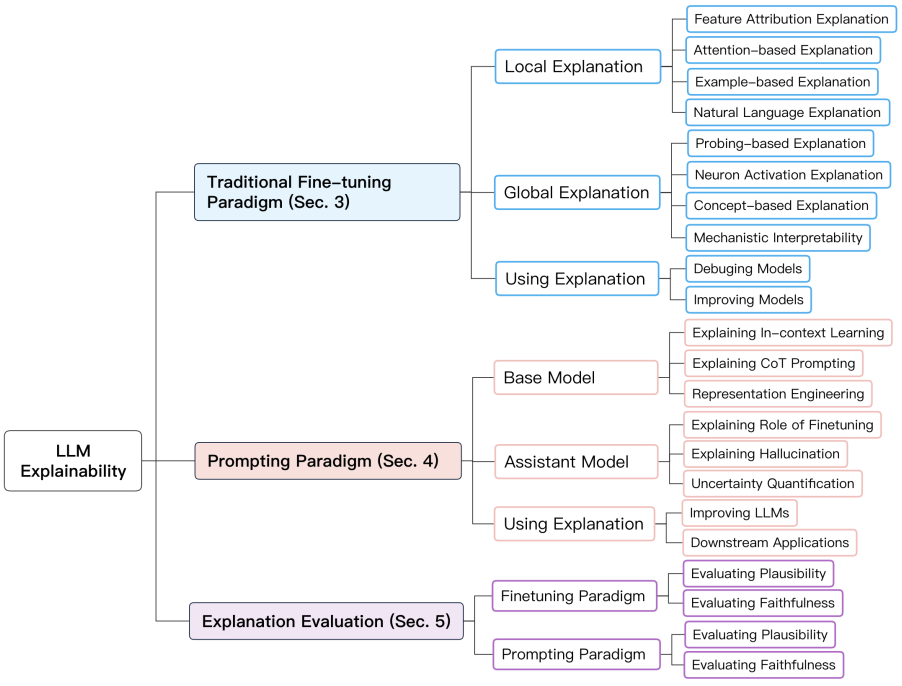
\includegraphics[width=1\textwidth]{figures/llm_explainability.png}
    \caption{Categories of LLM explainability adopted from \cite{zhao2023explainabilitylargelanguagemodels}} 
    \fxnote{Design own image}
    \label{fig:llm_explainability}
\end{figure}
The focus in the article is on the \textit{traditional fine-tuning paradigm}, more on that later. In this context, the key distinction between \textit{local explanation} and \textit{global explanation} is that the former aims to clarify individual model predictions, while the latter seeks to shed light on the internal workings of language models.
\\\\
The method introduced in the upcoming chapters falls under the \textit{local explanation} category and specifically under \textit{example-based explanation}, as it targets individual instances rather than isolated features \cite{zhao2023explainabilitylargelanguagemodels}.

\section{Problem Statement} \label{sec:problem_statement}
As mentioned above, this work focuses on example-based (instance-based) explanations. More specifically, the objective is to determine how effectively a model can identify the original data point given a paraphrased version of it. To that end, each sample in a supervised fine-tuning dataset is paraphrased and stored alongside its original counterpart. This paraphrasing is performed using an external model (GPT-4o mini \cite{openai_2024_gpt4o_mini}) or the model under evaluation. The original and paraphrased samples are then passed through the model, and the respective gradients for both samples are calculated. The cosine similarity is then employed to measure the degree to which these gradients align, providing a score between -1 and 1. The cosine similarity captures the cosine of the angle between two non-zero vectors, yielding a measure of similarity between the gradients. By comparing all gradients, we obtain a ranking and a corresponding score that indicate how well gradient-based explanations detect the original sample when given a paraphrased version for a given model.
\\\\
By using this method, the evaluation of these gradient-based explanations will not require a retraining of the model since it only computes how the model's output changes with respect to small changes in the input by paraphrasing. In simple terms, the original and paraphrased inputs are piped through the model and the difference of the respective gradients is measured. Hence, no additional training loop or parameter tuning is required. 
\\\\
While instance-based explanations are well known in the context of classification models, they have been relatively unexplored for \acrlong{llm}s. Given that \acrlong{llm}s can contain many parameters (for example, LLaMA 3.1 has up to 405 billion parameters \cite{meta_ai_llama_3_1}), the associated computations can be very expensive. Specifically, the proposed approach calculates at least one gradient for each layer per training sample. Consequently, for a single sample, the combined gradients can be as large as the entire model. In the case of LLaMA 3.1 (405B), the gradients of a single example contain up to 405 billion floating-point values.
\\\\
However, the proposed methodology contributes both a mechanism and a dataset to evaluate and benchmark instance-based explainability techniques. In addition, other explanation methods can be substituted for the gradient-based approach described here. Moreover, as already stated, this type of benchmark does not require retraining of the model, which makes it particularly well suited for already fine-tuned \acrshort{llm}s.

\subsection{Layer Importance}
Because \acrshort{llm}s incorporate numerous components, such as embedding, Transformer decoder, and \acrshort{mlp} layers \cite{Rosenblatt1958-mn}, it is beneficial to assess which layers have the greatest influence compared to all gradients of the layers. Here, we investigate how each layer influences both the ranking and the overall score of the attributions associated with the paraphrased samples.
\\\\
As already stated above, gradients of \acrshort{llm}s can be high-dimensional and hence expensive to work with. 

\fxnote[inline]{Further elaborate on layer selection, dimensionality reduction, other papers are just randomly picking layers (MLP)}

\fxnote[inline]{Size of gradients, random projections, layer importance, benefits of greedy selection etc. }
